% Generated by pysimcount.pfseeds -- do not edit; regenerate instead.
% figure: B-order4-by-formula -- Every order-4 formula at measured r; median over seeds [1, 2, 3, 4, 5, 6, 7, 8, 9, 10], bars = min..max
% metric=cnot gatebase=cz merged
% seed 1: git_commit=01d3c275ceae2840002bd1aaea68f59b987c4975 git_dirty=False
% seed 2: git_commit=01d3c275ceae2840002bd1aaea68f59b987c4975 git_dirty=False
% seed 3: git_commit=01d3c275ceae2840002bd1aaea68f59b987c4975 git_dirty=False
% seed 4: git_commit=01d3c275ceae2840002bd1aaea68f59b987c4975 git_dirty=False
% seed 5: git_commit=01d3c275ceae2840002bd1aaea68f59b987c4975 git_dirty=False
% seed 6: git_commit=01d3c275ceae2840002bd1aaea68f59b987c4975 git_dirty=False
% seed 7: git_commit=01d3c275ceae2840002bd1aaea68f59b987c4975 git_dirty=False
% seed 8: git_commit=01d3c275ceae2840002bd1aaea68f59b987c4975 git_dirty=False
% seed 9: git_commit=01d3c275ceae2840002bd1aaea68f59b987c4975 git_dirty=False
% seed 10: git_commit=01d3c275ceae2840002bd1aaea68f59b987c4975 git_dirty=False
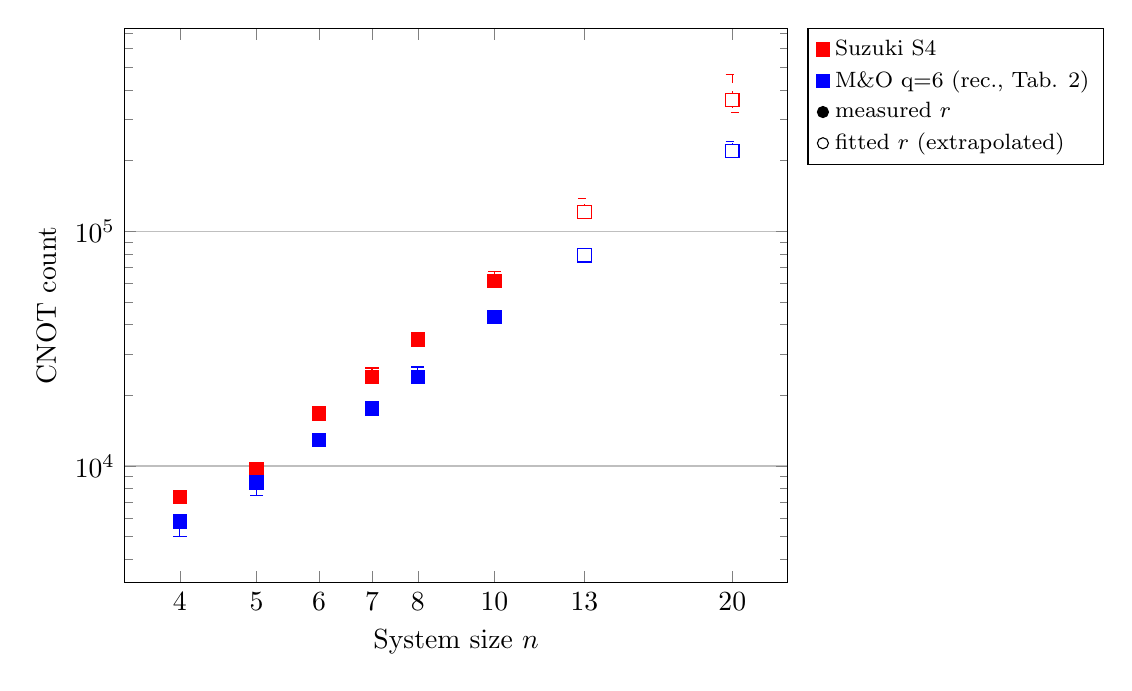
\begin{tikzpicture}
  \begin{loglogaxis}[
    width=10cm,
    xlabel={System size $n$},
    ylabel={CNOT count},
    xtick={4,5,6,7,8,10,13,20},
    xticklabels={4,5,6,7,8,10,13,20},
    ymajorgrids=true,
    legend pos=outer north east,
    legend cell align=left,
    legend style={font=\footnotesize},
  ]
    \addplot[only marks, red, mark=square*, mark size=2.4pt, mark options={solid, fill=red}, error bars/.cd, y dir=both, y explicit, error bar style={red}] coordinates {
      (4,7392) += (0,168) -= (0,0)
      (5,9660) += (0,420) -= (0,210)
      (6,16632) += (0,1260) -= (0,756)
      (7,23961) += (0,2205) -= (0,1323)
      (8,34608) += (0,1344) -= (0,1344)
      (10,61530) += (0,5670) -= (0,1470)
    };
    \addlegendentry{Suzuki S4}
    \addplot[only marks, red, mark=square*, mark size=2.4pt, mark options={solid, fill=white}, forget plot, error bars/.cd, y dir=both, y explicit, error bar style={red, dashed}] coordinates {
      (13,120939) += (0,17199) -= (0,7917)
      (20,363720) += (0,102480) -= (0,42000)
    };
    \addplot[only marks, blue, mark=square*, mark size=2.4pt, mark options={solid, fill=blue}, error bars/.cd, y dir=both, y explicit, error bar style={blue}] coordinates {
      (4,5800) += (0,200) -= (0,800)
      (5,8500) += (0,250) -= (0,1000)
      (6,12900) += (0,300) -= (0,600)
      (7,17675) += (0,875) -= (0,1225)
      (8,24000) += (0,2400) -= (0,1200)
      (10,43250) += (0,1750) -= (0,2750)
    };
    \addlegendentry{M\&O q=6 (rec., Tab. 2)}
    \addplot[only marks, blue, mark=square*, mark size=2.4pt, mark options={solid, fill=white}, forget plot, error bars/.cd, y dir=both, y explicit, error bar style={blue, dashed}] coordinates {
      (13,78975) += (0,5525) -= (0,1625)
      (20,219500) += (0,21500) -= (0,8500)
    };
    \addlegendimage{only marks, black, mark=*}
    \addlegendentry{measured $r$}
    \addlegendimage{only marks, black, mark=*, mark options={fill=white}}
    \addlegendentry{fitted $r$ (extrapolated)}
  \end{loglogaxis}
\end{tikzpicture}
